%%
%% This is file `sample-sigconf.tex',
%% generated with the docstrip utility.
%%
%% The original source files were:
%%
%% samples.dtx  (with options: `sigconf')
%% 
%% IMPORTANT NOTICE:
%% 
%% For the copyright see the source file.
%% 
%% Any modified versions of this file must be renamed
%% with new filenames distinct from sample-sigconf.tex.
%% 
%% For distribution of the original source see the terms
%% for copying and modification in the file samples.dtx.
%% 
%% This generated file may be distributed as long as the
%% original source files, as listed above, are part of the
%% same distribution. (The sources need not necessarily be
%% in the same archive or directory.)
%%
%% The first command in your LaTeX source must be the \documentclass command.
\documentclass[sigconf]{acmart}

\settopmatter{printacmref=false} % Removes citation information below abstract
\renewcommand\footnotetextcopyrightpermission[1]{} % removes footnote with conference information in first column
\pagestyle{plain}
% https://tex.stackexchange.com/a/176136
\newcommand{\vect}[1]{\boldsymbol{#1}}

%%
%% \BibTeX command to typeset BibTeX logo in the docs
\AtBeginDocument{%
  \providecommand\BibTeX{{%
    \normalfont B\kern-0.5em{\scshape i\kern-0.25em b}\kern-0.8em\TeX}}}

%% Rights management information.  This information is sent to you
%% when you complete the rights form.  These commands have SAMPLE
%% values in them; it is your responsibility as an author to replace
%% the commands and values with those provided to you when you
%% complete the rights form.
% \setcopyright{acmcopyright}
% \copyrightyear{2018}
% \acmYear{2018}
% \acmDOI{10.1145/1122445.1122456}

% %% These commands are for a PROCEEDINGS abstract or paper.
% \acmConference[Woodstock '18]{Woodstock '18: ACM Symposium on Neural
%   Gaze Detection}{June 03--05, 2018}{Woodstock, NY}
% \acmBooktitle{Woodstock '18: ACM Symposium on Neural Gaze Detection,
%   June 03--05, 2018, Woodstock, NY}
% \acmPrice{15.00}
% \acmISBN{978-1-4503-9999-9/18/06}


%%
%% Submission ID.
%% Use this when submitting an article to a sponsored event. You'll
%% receive a unique submission ID from the organizers
%% of the event, and this ID should be used as the parameter to this command.
%%\acmSubmissionID{123-A56-BU3}

%%
%% The majority of ACM publications use numbered citations and
%% references.  The command \citestyle{authoryear} switches to the
%% "author year" style.
%%
%% If you are preparing content for an event
%% sponsored by ACM SIGGRAPH, you must use the "author year" style of
%% citations and references.
%% Uncommenting
%% the next command will enable that style.
%%\citestyle{acmauthoryear}


\usepackage{caption}
\usepackage{amsmath}
\usepackage{amssymb}
\usepackage{dsfont}
\usepackage{hyperref}


% Caption setup for multiline caption
% See: https://tex.stackexchange.com/questions/247409/centered-captionlabel-above-justified-caption-text
% Modified to my needs.
\DeclareCaptionFormat{center}{#1#2#3}
\captionsetup{format=center, justification=justified}

% where to put all images and figures
\graphicspath{{images/}}




%%
%% end of the preamble, start of the body of the document source.
\begin{document}

%%
%% The "title" command has an optional parameter,
%% allowing the author to define a "short title" to be used in page headers.
\title{Bridging the gap between variational autoencoders and adversarial attack.}

%%
%% The "author" command and its associated commands are used to define
%% the authors and their affiliations.
%% Of note is the shared affiliation of the first two authors, and the
%% "authornote" and "authornotemark" commands
%% used to denote shared contribution to the research.
\author{Lorenz Hofmann-Wellenhof}
\email{hofmannw@fim.uni-passau.de}

%%
%% The abstract is a short summary of the work to be presented in the
%% article.
\begin{abstract}
  Deep neural networks are the base for variational autoencoders and both show
  excellent performance in many areas. However, they are vulnerable to
  adversarial attacks, that are elaborately designed perturbations to the input
  data, that fool the model at inference time. In this work we present an
  overview of variational autoencoders and adversarial examples and methods to
  combine both areas.
\end{abstract}

%%
%% Keywords. The author(s) should pick words that accurately describe
%% the work being presented. Separate the keywords with commas.
\keywords{autoencoders, adversarial examples, deep learning, deep generative models}


%%
%% This command processes the author and affiliation and title
%% information and builds the first part of the formatted document.
\maketitle

\section{Introduction}\label{sec:introduction}
Deep neural networks have become significantly useful at many difficult machine
learning tasks. They are able to recognize images with near human accuracy
\cite{lecun1998gradient}. They are used for speech recognition
\cite{hinton2012deep}, natural language processing \cite{andor2016globally}, and
playing games \cite{silver2016mastering}.

Deep neural networks are the foundation of deep generative models which are
among the most promising approaches. Generative models have many short-term
applications like image generation \cite{goodfellow2014generative}, text
generation \cite{semeniuta2017hybrid}, or semi- and unsupervised machine
learning tasks \cite{radford2015unsupervised}  but in the long run, they hold
the potential to automatically learn the natural features of a dataset, whether
categories or dimensions or something else entirely.

One of the most popular generative model is the variational autoencoder (VAE)
for unsupervised learning of complicated distributions. VAE are tempting,
because they build on top neural network, can be trained with stochastic
gradient descent. VAEs have already shown promise in generating many kinds of
complicated data, including handwritten digits, faces, house numbers, CIFAR
images, physical models of scenes, and segementation.

However, researchers have discovered that existing neural networks are
vulnerable to attack. The goal of adversarial attacks is to fool deep neural
networks by applying elaborately designed perturbation to input data.
Adversarial attacks make it dangerous to use deep neural networks in
applications in the real world. In the case of autonomous driving, by making an
object detector recognize pedestrians as roads, attacks can cause an accident.

The existence of adversarial examples has inspired research into how neural
networks can be hardened against such attacks. Defensive distillation is one of
those recently proposed defenses to harden neural networks against adversarial
examples. Initial analysis was very promising: defensive distillation defeats
existing attack algorithms and reduces their likelihood of success from 95\% to
0.5\%. Defensive distillation can be applied to any feed-forward neural network
and requires only one retraining step, and is currently one of the only defenses
that offers strong safety guarantees against examples of adversaries.

In this paper an overview is given on the different kinds of autoencoders and
variational autoencoders. Then prominent adversarial attacks are outlined. At
last, we take a look at recent work that combines VAE and adversarial methods.
Contributions in relations with this paper are listed in section
\ref{sec:adversarial_attacks}.
\section{Autoencoder}\label{sec:autoencoder}
This section starts with describing the basic philosophy of an autoencoder and
then takes a look at different types of autoencoders.

An autoencoder is a neural network trained to copy its input to its output
\cite{Goodfellow-et-al-2016}. It has a hidden layer \textbf{h} internally that
specifies a code used to represent the input. The network can be viewed as being
composed of two parts: an encoder function $\textbf{h} = f(\textbf{x})$ and a
decoder producing the reconstruction $\textbf{r} = g(\textbf{h})$. The general
structure of autoencoders can be seen in Figure \ref{fig:autoencoder}.

If an autoencoder is able to learn to set $g(f(\textbf{x}))=\textbf{x}$
anywhere, it is not particularly useful. Rather, autoencoders are designed to be
unable to learn how to copy perfectly. Usually they are restricted in ways that
only approximately allow them to copy. Additionally, it can handle only input
that is similiar to the training data. Since the model is forced to prioritize
which input features are to be copied, it often learns useful data characteristics. 

For decades, the idea of autoencoders has been part of neural networks' history.
Autoencoders have traditionally been used to reduce dimensionality or to learn
features. Recently, connections between latent variable models and autoencoders
brought up autoencoders as a cutting edge technology for generative modeling.
Autoencoders can be considered as a special case of feedforward networks and can
be trained with the same techniques, typically minibatch gradient descent after
gradients calculated by back-propagation. 

\begin{figure}[h]
    \centering
    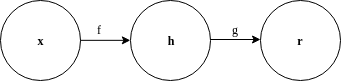
\includegraphics[width=\linewidth]{/1_introduction/autoencoder}
    \caption{An autoencoder's general structure, mapping an input $\textbf{x}$
    to an output (reconstruction) $\textbf{r}$ by an internal representation or
    code $\textbf{h}$. There are two components in the autoencoder: the encoder
    $f$ (mapping $\textbf{x}$ to $\textbf{h}$) and $g$ (mapping $\textbf{h}$ to
    $\textbf{r}$).}
    \label{fig:autoencoder}
\end{figure}


\subsection{Undercomplete Autoencoders}
Copying the input to the output may sound useless, but we are usually not
concerned about the decoder's output. Instead, by training the autoencoder we
try to achieve that $ \textbf{h}$ is taking on useful features, as a result of
copying the input to the output \cite{vincent2010stacked}.

To obtain useful features from the autoencoder we define $\textbf{h}$ with a smaller size
than $\textbf{x}$. \textbf{Undercomplete} autoencoders have a code dimension
which is smaller than the input dimension. Learning an undercomplete
representation causes the autoencoder to capture the training data's most
important features. 

We can describe this learning process as minimizing a loss function
\begin{equation}
    L(\textbf{x}, g(f(\textbf{x}))),
\end{equation}
where L is a loss function that penalizes $g(f(\textbf{x}))$ as being dissimilar
to $\textbf{x}$, such as the mean squared error. 

An undercomplete autoencoder learns to span the same subspace as principal
component analysis (PCA) when the decoder is linear and $L$ is the mean squared
error. In this case, as a side effect the autoencoder learned the prinicipal
suspace of the training data while performing training.

Thus, autoencoders with nonlinear encoder functions $f$ and nonlinear decoder
functions $g$ can learn to generalize PCA more powerfully. However, if too much
capacity is permitted for the encoder and decoder, the autoencoder might learn to
perform the copying task without extracting useful features from the data. 

\subsection{Regularized Autoencoders}
An akin problem happens when the hidden code has dimensions equal to the input,
or dimensions larger than the input. Under those circumstances, even a linear
encoder and a linear decoder learns how to replicate the input to the output
without learning anything meaningful about the distribution of the data  
\cite{makhzani2015adversarial}.

Ideally, any autoencoder architecture could be successfully trained by choosing
the code dimension and the encoder and decoder capacity based on the complexity
of the distribution to be modeled. Regularized autoencoders support this
capability. Instead of restricting the capacity of the model by keeping the
encoder and decoder shallow and code size small, regularized autoencoders use a
loss function that advocates the model to have other aspects than to copy its
input to its output. These other aspects include sparsity of representation,
smallness of representation derivative, and robustness to noise or missing
inputs. 

In conjuction with the methods explained here, which are interpreted most
naturally as regularized autoencoders, almost any generative model with latent
variables and equipped with an inference procedure (for computing latent
representations given input) can be understood as a particular form of
autoencoder. Variational autoencoders are another generative modeling approach
that emphasizes this relation with autoencoders. Naturally, these models learn
high-capacity, overcomplete input encodings and do not neeed regularization to
be useful. Their encoding is naturally effective as the models have been trained
to approximately maximize the probability of training data rather than copying
the input to the output. 

\subsection{Stochastic Encoders and Decoders}
Autoencoders are feedworward networks. The same loss functions and output unit
types that are used for traditional feedforward networks can be applied for
autoencoders aswell.

A general strategy for the design of the output units and the feedforward
network loss function is to define the output distribution
$p(\textbf{y}|\textbf{x})$ and minimize the negative log-likelihood $-\log
p(\textbf{y}|\textbf{x})$ . In that case \textbf{y} is a vector of targets, such
as class labels \cite{werbos2002stochastic}.

We may think of the decoder as a conditional distribution \\
$p_{decoder}(\textbf{x}|\textbf{h})$ given a hidden code $\textbf{h}$. Then, by
minimizing 
\begin{equation}
    -\log p_{decoder}(\textbf{x}|\textbf{h})
\end{equation}
we can train the autoencoder. The exact shape of this loss function depends on
the shape of \textbf{p}. Additionally, we can generalize the notion of an
\textbf{encoding function} $f(\textbf{x})$ to an \textbf{encoding distribution}
$p_{encoder}(\textbf{h}|\textbf{x})$.

\begin{figure}
	\centering
	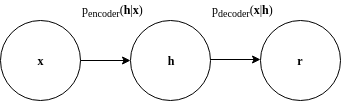
\includegraphics[width=\linewidth]{/1_introduction/autoencoder_stochastic}
    \caption{The architecture of a stochastic autoencoder, in which both the
    encoder and the decoder are not simple functions. Their output can be seen
    as samples from a distribution, $p_{encoder}(\textbf{h}|\textbf{x})$ for the
    encoder and $p_{decoder}(\textbf{x}|\textbf{h})$ for the decoder.}
\end{figure}

\subsection{Variational Autoencoders} \label{subsec:varautoencoders}
Many generative models form on the idea of using a differentiable generator
network. The model uses a differentiable function that is typically defined by a
neural network to convert samples of latent variables \textbf{z} into samples
\textbf{x} or distributions over samples \textbf{x}. This model class combines
autoencoders that match the generator net with an inference net (encoder)
\cite{doersch2016tutorial}.

To create a sample from the model, the VAE first picks a sample \textbf{z}
from the code distribution $p_{model}(\textbf{z})$. Then the sample runs through
a differentiable generator network $g(\textbf{z})$. At last, \textbf{x} is
sampled from a distribution $ p_{model}(\textbf{x};g(\textbf{z})) =
p_{model}(\textbf{x}|\textbf{z})$. During training, the encoder
$q(\textbf{z}|\textbf{x})$ is used to obtain \textbf{z}, and
$p_{model}(\textbf{x}|\textbf{z})$ is then viewed as decoder network. The
architectural overview of an variational autoencoder is visualized in Figure
\ref{fig:autoencoder_architecture}.

The key observation behind variational autoencoders is that they can be trained by
maximizing the variational lower bound $\mathcal{L}(q)$ associated with data
point \textbf{x}:

\begin{figure}
	\centering
	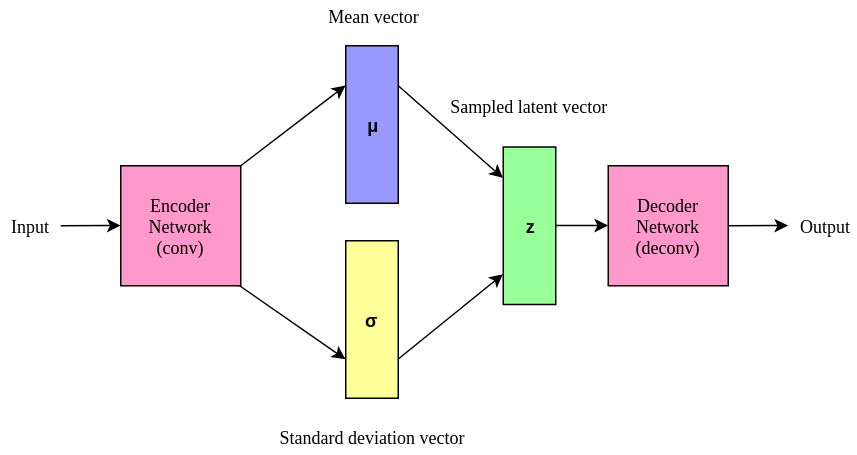
\includegraphics[width=\linewidth]{/2_background/variational_autoencoder_architecture}
    \caption{The architectural overview of a variational autoencoder. On the
    left side is the encoder which is typically a convolutional neural network.
    In the middle we see the standard deviation and the mean of the distribution
    $q(z|x)$ which are optimized during training. Following with the sampled
    latent vector z and the decoder $p_{model}(x|z)$ containing the generator
    network $g(z)$.} 
	\label{fig:autoencoder_architecture}
\end{figure}

\begin{flalign}
    \mathcal{L}(q)  &= \mathds{E}_{z \sim q(\textbf{z}|\textbf{x})} \log p_{model}(\textbf{z}, \textbf{x}) + \mathcal{H}(q(\textbf{z}|\textbf{x})) \label{vae:1} && \\
                    &= \mathds{E}_{z \sim q(\textbf{z}|\textbf{x})} \log 
                    p_{model}(\textbf{x}|\textbf{z}) -
                    D_{KL}(q(\textbf{z}|\textbf{x})||p_{model}(\textbf{z})) \label{vae:2} && \\
                    &\leq \log p_{model}(\textbf{x}).
\end{flalign}

In equation \ref{vae:1}, the first term outlines the expected value of the joint
log-likelihood of the visible and hidden variables with respect to the
probabilty distribution $q(\textbf{z}|\textbf{x})$ (approximate posteriror). The
second term defines the entropy of the approximate posterior. The entropy term
encourages the variational posterior to place high probabilty mass on many
\textbf{z} values that could have generated \textbf{x}, rather than collapsing
to a single point estimate of the most likely value.

In equation \ref{vae:2} we describe the first term as the reconstruction
log-likelihood used in other autoencoders. The second term makes the posterior
distribution $q(\textbf{z}|\textbf{x})$ and the model prior
$p_{model}(\textbf{z})$ distribution approach each other. This is accomplished with the
Kullback-Leibler divergence which is a measure of how one probability
distribution is different from a second.

The main intuition behind the variational autoencoder is to train an encoder that
produces the parameters of $q$. As long as $\textbf{z}$ is a continuous
variable, it is possible to back-propagate through the samples (by using the
reparameterization trick) of $\textbf{z}$ drawn from $q(\textbf{z}|\textbf{x}) =
q(\textbf{z};f(\textbf{x};\boldsymbol\theta))$ to obtain a gradient with respect
to $\boldsymbol\theta$, where $\boldsymbol\theta$ defines the model parameters
of the VAE.

VAE achieves excellent results and is one of the state-of-the-art generative
modeling approaches. The main disadvantage is that samples from variational
autoencoders trained on images are likely to be a little bit blurry. It is not
yet known why this anomaly happens. One possibility is that the blurriness is an
instrinsic effect of maximum likelihood \cite{Goodfellow-et-al-2016}.

\subsubsection{Reparameterization trick}
Traditional neural networks execute a deterministic conversion of some input
variables \textbf{z}. When using VAE or other generative models, it is necessary
that neural networks implement a stochastic conversion of \textbf{z}.
However, it is not possible to backpropagate through a stochastic node. One
simple solution is to augment the neural network with extra inputs
$\boldsymbol\epsilon$ that are sampled from a simple probability distribution.
The neural network can then continue to perfrom deterministic computation
internally like calculating gradients for training using back-propagation
\cite{kingma2015variational}.

As an example let us look at the operation of generating a sample from a VAE.
During training the VAE model draws a sample \textbf{z} from
$q(\textbf{z}|\textbf{x})$, which might be a Gaussian distribution with mean
$\mu$ and variance $\sigma^2$.

\begin{equation}
    z \sim \mathcal{N}(\mu, \sigma^2).
\end{equation}

Because an individual sample of z is not created by a function, but rather by a
sampling process whose output changes every time we query it, it may seem
counterintuitive to take the derivatives of $\vect{z}$ with respect to the parameters of
its distribution, $\mu$ and $\sigma^2$. However, we can rewrite the sampling
process as transforming an underlying random value $\epsilon \sim
\mathcal{N}(\epsilon; 0, 1)$ to obtain a sample from the desired distribution:

\begin{equation}
    z = \mu + \sigma * \epsilon.
\end{equation}

Now it is possible to back-propagate through the sampling operation, by
regarding it as a deterministic operation with an extra input $\epsilon$.
Figure \ref{reparam_trick} visualizes the reparameterization trick.

\begin{figure}
	\centering
	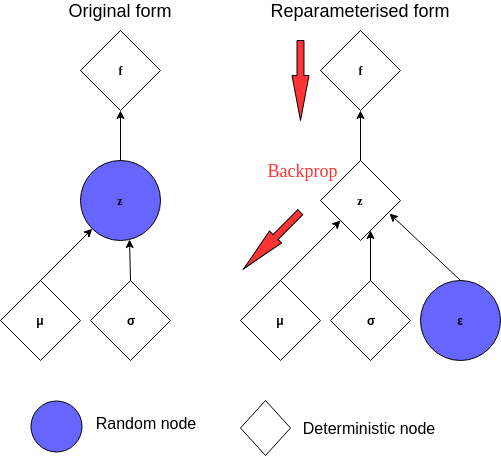
\includegraphics[width=\linewidth]{/2_background/reparam_trick}
    \caption{On the left hand side the original form is displayed. It is not
    possible to back propagate through a stochastic node. On the right side the
    reparameterised form is displayed with a stochastic node $\epsilon$ giving
    the opportunity to train parameters $\mu$ and $\sigma$ while
    back-propagation.} 
	\label{reparam_trick}
\end{figure}

\section{Adversarial Attacks}\label{chap:state-of-the-art}

Many machine learning models, including neural networks, consistently
misclassify adversarial examples - inputs formed by applying small but
intentionally worst-case perturbations to examples from the dataset, such that
the perturbed input results in the model outputting an incorrect answer with
high confidence \cite{goodfellow2014explaining}. An adversarial example is
described as

\begin{equation}
    \vect{x}^{adv}  = \vect{x} + \vect{\eta}.
\end{equation}

Where $\vect{x}^{adv}$ is the adversarial example, $x$ the original input and $\eta$
the perturbation.


First, this section describes the most promiment methods (attacks) to generate
adversarial examples and then highlights efforts that have been made to connect
adversarial examples with autoencoders. The attacks mentioned here can be found
in the cleverhans\footnote{github.com/tensorflow/cleverhans} library.
Contributions to the library in relation with this paper can be found here\footnote{github.com/tensorflow/cleverhans/pull/1037}
and here\footnote{github.com/tensorflow/cleverhans/pull/1047}.

\subsection{Fast Gradient Sign Method}
The "fast gradient sign method" (FGSM) refers to an attack that computes the
perturbation $\eta$ by calculating:

\begin{equation}\label{eq:fgsm}
    \vect{\eta} = \epsilon * sign(\nabla_x J (\vect{\theta}, \vect{x}, y)).
\end{equation}

Where $\vect{\theta}$ are the parameters of a model, $\vect{x}$ the input to the
model, $y$ the targets associated with $\vect{x}$ (for machine learning tasks
that have targets) and $J(\vect{\theta}, \vect{x}, y)$ the loss used to train
the neural network. Equation \ref{eq:fgsm} linearizes the cost function around
the current value of $\vect{\theta}$, obtaining an optimal max-norm constrained
pertubation $\vect{\eta}$. The elements of $\vect{\eta}$ are equal to the sign of
the elements of the gradient of the loss function with respect to the input.
$\epsilon$ is a number big enough such that the adversarial example is
effective, but small enough such that it won't be noticed in the generated
example. Figure \ref{fig:fgsm_panda} \cite{goodfellow2014explaining} visualizes
the effect of FGSM.


\begin{figure}
	\centering
	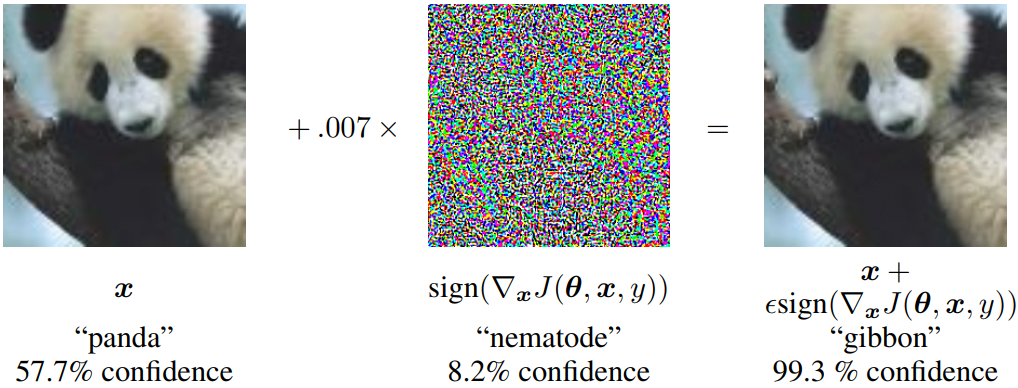
\includegraphics[width=\linewidth]{/3/fgsm_panda}
    \caption{FGSM applied to GoogLeNet \cite{szegedy2015going} on ImageNet. By
    adding an inconspicuous pertubation to the original image, GoogLeNet's
    classification of the image can be changed.} 
	\label{fig:fgsm_panda}
\end{figure}

\subsection{Projected Gradient Descent}
A straightforward way to enhance FGSM is, to apply it multiple times with a
small step size, and clip pixel values of intermediate results after each step
to make sure that they are in an $\epsilon-neighbourhood$  of the original
image:


\begin{equation}\label{eq:fgsm}
    \vect{x}^{adv}_{0} = \vect{x}, \quad \vect{x}^{adv}_{N + 1}=Clip_{x, \epsilon} \Big \{\vect{x}^{adv}_{N} + \alpha sign\big(\nabla_{x}J(\vect{x}^{adv}_{N}, y)\big)  \Big\}
\end{equation}

Typcially $\alpha = 1$ is used. This means that value of each poxel is only
changed by 1 on each step. This method is known as "projected gradient descent"
(PGD) or "basic iterative method". \cite{kurakin2016adversarial, madry2017towards}
\section{Autoencoders and Adversarial Examples}\label{sec:combining}
In this section we take a look at work that combines adversarial examples and
variational autoencoders.

\subsection{Adversarial Images for Autoencoder}
This approach \cite{tabacof2016adversarial} describes a method for creating a
distortion based on variational autoencoders: Our attack consists of selecting
an original image and a target image and then feeding the network with the
original image added to a small distortion, optimized to get the result as close
as possible to the target image (Figure
\ref{fig:adversarial_images_autoencoder}). Autoencoders reconstruct from the
latent representation, which makes it the information bottleneck, and therefore
particularly convenient to attack. The authors used the following adversarial
optimization:
    
\begin{align}
    & \min_{d} \quad \Delta(\vect{z}_{a}, \vect{z}_{t}) + C||\vect{d}|| && \\
    & s.t. \quad  
        \begin{aligned}[t]
            & L \leq \vect{x} + \vect{d} \leq U \\
            & \vect{z}_a = encoder(\vect{x} + \vect{d})
        \end{aligned}
\end{align}

\begin{figure}
	\centering
	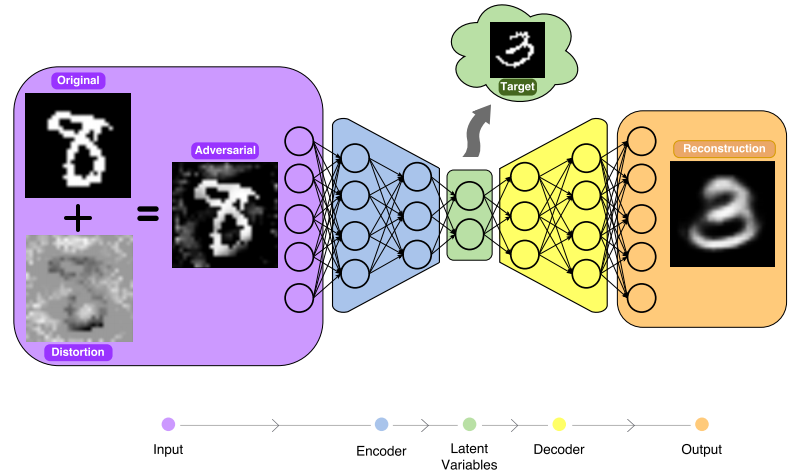
\includegraphics[width=\linewidth]{/4/adversarial_images_autoencoder}
    \caption{Adversarial attacks for autoencoders apply distortions to the input
    with goal of having the autoencoder reconstruct another target. The latent
    representation is attacked, by attempting to match it to the target image's
    \cite{tabacof2016adversarial}.} 
	\label{fig:adversarial_images_autoencoder}
\end{figure}

where $\vect{d}$ is the adversarial distortion; $\vect{z}_{a}$ and
$\vect{z}_{t}$ are the latent representations of the adversarial and the target
images; $\vect{x}$ is the original image; $\vect{x} + \vect{d}$ is the
adversarial image; $L$ and $U$ are bounds on the input space; and C is the
regularizing constant that balances reaching the target and limiting the
distortion.

For variational autoencoders $\Delta$ is chosen as the the KL-divergence to
measure the difference between the two probabilty distributions. $z_{*}$
correspond to uncorrelated multivariate normal distributions with parameters
given by the encoder:

\begin{equation}
    encoder(\vect{x}) \sim \mathcal{N}\big(\vect{M}_{\theta}(\vect{x}), \vect{\Sigma}_{\theta}(\vect{x})\big)
\end{equation}

where $\vect{M}$ and $\vect{\Sigma}$ represent the mean vector, and the
covariance matrix outputted by the last layer of the encoder network; $\theta$
are the autoencoder parameters \---- learned previously by training it for its
ordinary task of reconstruction. During the entire adversarial optimization,
$\theta$ remains fixed.

Results of this experiment show that generating adversarial images for
autoencoders is a much harder task than for classifiers. If a little distortion
(comparable to those used for misleading classifiers) is applied, the
reconstruction stays almost untouched. To get reconstructions very close to the
target's, it is necessary to add heavy distortions to the input. However, by
hand-tuning the regularization parameter, it is possible to find trade-offs
where the reconstruction approaches the target's and the adversarial image will
still look like the input.

\subsection{Purify Adversarial Examples with PuVAE}
\begin{figure}
	\centering
	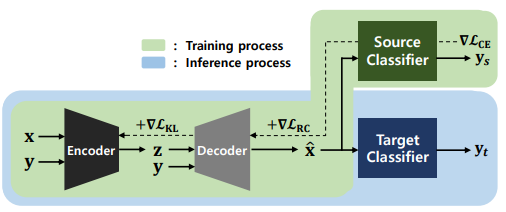
\includegraphics[width=\linewidth]{/4/puvae_1}
    \caption{Overview of the PuVAE algorithm; The green region shows the trainin
    process, and the blue region denotes the inference process of PuVAE. The
    dotted line represents the gradient flow during training. The parameters off
    the source classifier are not updated \cite{hwang2019puvae}.} 
	\label{fig:puvae_1}
\end{figure}

Authors of this paper \cite{hwang2019puvae} introduced a defense mechanisms
based on variational autoencoders. They propose Purify Variational Autoencoder
(PuVAE), a method to purify adversarial examples. The proposed method eliminates
an adversarial perturbation by projecting an adversarial example on the manifold
of each class, and determines the closest projection as a purified sample.

\subsubsection{Training PuVAE}
A data set $\mathcal{X}$ is defined which contains clean samples and adversarial
examples. Similiar as explained in subsection \ref{subsec:varautoencoders} the
authors trained PuVAE by maximizing the variational lower bound associated with
a datapoint $x$ from $\mathcal{X}$. Additionally, a cross-entropy calculated
from a classifier is used as a loss function for PuVAE. The classifier, called
\textit{source} classifier $M_{s}$, learns the decision boundaries on the data
space. The trained $M_{s}$ is used to ensure that the output instance reflects
the characteristics of the classes in the dataset. The cross-entropy loss from
$M_{s}$ is as follows:

\begin{equation}
    \vect{y}_{s} = M_{s}(\hat{\vect{x}})
\end{equation}
\begin{equation}
    \mathcal{L}_{CE} = \vect{y}_{data} \log \vect{y}_{s} + (1 - \vect{y}_{data}) \log (1 - \vect{y}_s)
\end{equation}

Finally, the PuVAE is trained using stochastic gradient descent:

\begin{equation}
    \nabla(\lambda_{RC} \mathcal{L}_{RC} + \lambda_{KL} \mathcal{L}_{KL} + \lambda_{CE} \mathcal{L}_{CE})
\end{equation}

where $\mathcal{L}_{RC}$ denotes the reconstruction loss and $\mathcal{L}_{KL}$
denotes the Kullback-Leibler divergence (both described in equation \ref{vae:2})
and $\mathcal{L}_{CE}$ the loss from the $M_{s}$ classifier. Figure
\ref{fig:puvae_1} gives an overview of the training process of PuVAE.


\subsubsection{Generating Purified Samples}
During inference time, the PuVAE projects an input sample to the data manifolds
of all classes in the dataset as follows:

\begin{equation}
    \hat{\vect{x}}_{y_i} = PuVAE(x, \vect{y_{i}})
\end{equation}

where $\vect{y}_i$ denotes the i-th class label to guide the input to the
corresponding latent space, and $\hat{\vect{x}}_{y_i}$, denotes a candidate for
the purified sample. Because PuVAE only learns the distribution of $\vect{z}$
from the training data, the input is mapped to the learned latent spaces even if
adversarial examples come in. The adversarial perturbations are removed in the
projection to the latent variable.

Then, the class label $y^*$ corresponding to the closest projection is selected as follows:

\begin{equation}
    \vect{y^*} = argmin_{y_{i} \in C} D(\vect{x}, \hat{\vect{x}}_{i})
\end{equation}

where $D$ denotes a distance measure to determine the closest projection and $C$
is the set of all possible class labels. The authors used the root mean square
error as the distance measure. Therefore, the candidate generated with label
$\vect{y}^*$ is the purified sample which goes into $M_{t}$:

\begin{equation}
    \vect{x}_{purified} = \hat{\vect{x}}_{y^*}
\end{equation}

At last, the purified sample is processed by the target classifier $M_{t}$ as follows:

\begin{equation}
    \vect{y}_{t} = M_{t}(\vect{x}_{purified})
\end{equation}

The authors test the robustness of PuVAE against various attack methods. PuVAE
exihibit performances competitive with state-of-the-art defense methods, and the
inference time is approximately 130 times faster than that of Defense-GAN that
is the state-of-the art purifier model.
\section{Conclusion}
TODO


  % Some examples.  A paginated journal article \cite{Abril07}, an
  % enumerated journal article \cite{Cohen07}


 
%%
%% The acknowledgments section is defined using the "acks" environment
%% (and NOT an unnumbered section). This ensures the proper
%% identification of the section in the article metadata, and the
%% consistent spelling of the heading.


%%
%% The next two lines define the bibliography style to be used, and
%% the bibliography file.
\bibliographystyle{bibliography/ACM-Reference-Format}
\bibliography{bibliography/sample-base}

%%
%% If your work has an appendix, this is the place to put it.
% \appendix

% \section{Research Methods}

% \subsection{Part One}

% \subsection{Part Two}

% \section{Online Resources}

\end{document}
\endinput
%%
%% End of file `sample-sigconf.tex'.
